\documentclass[12pt]{article}
\usepackage{ceai} % Uncomment this and remove the block above to use your custom package.
\graphicspath{{../figs/}}
\begin{document}
\doublespacing	

\title{CE 488/5588: Applied AI for Engineering\\ \large Topic 1: Intelligence: How to Equip a Machine with Intelligence}
\author{}
\date{}
\maketitle

\begin{ch-box}
As a starting point, before diving into specific AI methods, we raise a fundamental question: to what extent can intelligence be instantiated, approximated, or operationalized in artificial systems?
\end{ch-box}

\section{From Primitive Cognition to Human Intelligence}
Intelligence is often intuitively regarded as a uniquely human attribute, emerging from human cognition, consciousness, and lived experience. From this perspective, the notion of equipping a machine with intelligence appears, at first glance, both conceptually challenging and technically ambitious. Upon closer examination, however, this intuition proves incomplete. Intelligence is not exclusive to humans, nor does it manifest in a single, monolithic form.

While no rigorous, universally accepted scale exists for measuring intelligence across biological and artificial systems, qualitative comparisons of diverse organisms reveal a broad spectrum of intelligent behavior. These range from primitive, stimulus-driven responses to highly abstract reasoning and long-term planning. Examining such examples helps us contextualize contemporary AI systems within the broader landscape of intelligence.

\begin{itemize}
    \item \textit{Paramecium}. A paramecium is a single-celled organism lacking a nervous system, yet it exhibits surprisingly adaptive behavior. Through cilia-based locomotion and chemical sensing, it can move toward nutrients, avoid harmful stimuli, and adjust its motion based on environmental feedback. These behaviors emerge from biochemical and biophysical processes rather than symbolic reasoning, demonstrating that adaptive intelligence can arise without neurons, memory, or consciousness.

    \item \textit{Ant Colony}. Individual ants possess extremely limited cognitive capabilities, often following simple local rules such as pheromone tracking or obstacle avoidance. However, when operating collectively, ant colonies demonstrate emergent intelligence: efficient foraging, adaptive path planning, dynamic task allocation, and primitive forms of optimization. This highlights that intelligence can be distributed across interactions rather than centralized in a single individual.

    \item \textit{American Crows and African Greys}. These birds exhibit advanced cognitive abilities, including tool use, causal reasoning, episodic-like memory, and symbolic communication. African Grey parrots, for example, can learn abstract concepts such as color, shape, and number, while crows demonstrate multi-step planning. These abilities suggest that sophisticated reasoning can evolve independently of primate brain structures.

    \item \textit{Orangutans}. Orangutans display high-level intelligence comparable to early hominins, including long-term planning, social learning, deception, and tool construction. They can mentally simulate future scenarios—such as preparing tools for later use—indicating the presence of internal world models and intentional reasoning.
\end{itemize}

From these examples, we observe that intelligence spans a vast spectrum: from reflexive, embodied responses in single-celled organisms, to emergent collective intelligence in social insects, to abstract reasoning in higher animals. Intelligence is therefore not a singular property, but a collection of capabilities, including sensing, perception, learning, memory, adaptation, prediction, and decision-making—realized through radically different physical substrates.

A critical implication of this diversity lies in the concept of \textit{embodied intelligence}. Even a single-celled paramecium can autonomously sense its environment, navigate complex fluid spaces, acquire energy, avoid threats, and reproduce. In stark contrast, modern artificial systems remain extremely limited in this regard. No existing AI possesses this full closed loop of perception, action, survival, and self-sustenance.


For the purposes of engineering artificial systems, we adopt an operational rather than philosophical definition of intelligence. In this course, intelligence refers to the ability of a system to acquire internal representations from experience and to use those representations to predict, decide, and act under uncertainty in pursuit of specified objectives. This definition does not assume consciousness, understanding, or intentionality; instead, it emphasizes functional capability and performance within a well-defined environment. Under this definition, machine learning (ML), as discussed later, is a dominant subset of AI and provides a practical mechanism for constructing such representations and decision rules when explicit modeling of the environment is infeasible or incomplete.


% Most AI systems today operate as input--output machines: given sensory data (images, text, signals), they compute an output (classification, prediction, control signal) according to a learned or programmed function. Regardless of complexity—from a simple regression model to a trillion-parameter neural network—these systems remain fundamentally end-to-end mappings with limited autonomy, no intrinsic goals, and no genuine understanding of their physical existence.

Consequently, contemporary AI can be viewed as an extremely powerful calculator. While it may possess vast encoded knowledge and remarkable pattern-matching abilities, it lacks intrinsic intentionality or survival-driven agency. These systems excel at domains of intelligence that are relatively formalizable and well-constrained, such as logic, mathematics, pattern recognition, and structured language use, because these domains admit stable representations, large static datasets, and objective performance metrics. While these problems are not intrinsically simple, they are amenable to large-scale optimization and statistical learning.


By contrast, intelligence in open-ended, embodied settings—such as physical survival, continual adaptation under uncertainty, and autonomous goal management—remains largely unsolved. These settings involve non-stationary environments, incomplete feedback, long time horizons, and tight perception–action coupling, which challenge current learning paradigms.

This contrast reflects a broader pattern observed in cognitive science and robotics: tasks that are effortless for biological organisms often prove difficult for machines, whereas tasks that require formal reasoning are comparatively easier to mechanize.


Given this vast scope of AI, we must narrow our focus. In this course, we concentrate on the forms of intelligence that machines can reliably realize today. To do so, we first examine the fundamental reasoning processes humans adopt in decision-making, which serve as the blueprint for modern AI architectures.

\section{Decision-Making and Reasoning}
Decision-making and problem-solving are central to the human experience. At the foundation of these activities lies \textit{reasoning} - the cognitive process by which information is interpreted, generalized, and applied to guide action. Over centuries of inquiry in philosophy, logic, and cognitive science, several fundamental forms of reasoning have been identified, including deductive, inductive, abductive, and analogical reasoning.

Modern AI and machine learning (ML) models embody elements of these reasoning processes in algorithmic form. It is important to emphasize that machine `reasoning' is fundamentally different from human cognition: artificial systems operate through silicon-based computation and formal optimization, whereas human reasoning emerges from biological processes and lived experience. Nevertheless, drawing analogies between human reasoning and machine computation provides a useful conceptual lens.

A defining characteristic of human intelligence is the continuous cycle between reasoning modes. Humans often \textit{induce} general principles from experience and observation, then apply those principles \textit{deductively} to novel situations. This inductive--deductive loop underlies scientific discovery, engineering design, and everyday decision-making. Contemporary AI systems largely operate within this same conceptual loop.

We focus here on four primary reasoning types, with particular emphasis on deduction and induction, as they form the backbone of classical and modern AI methodologies.

\begin{figure}[ht]
    \centering
    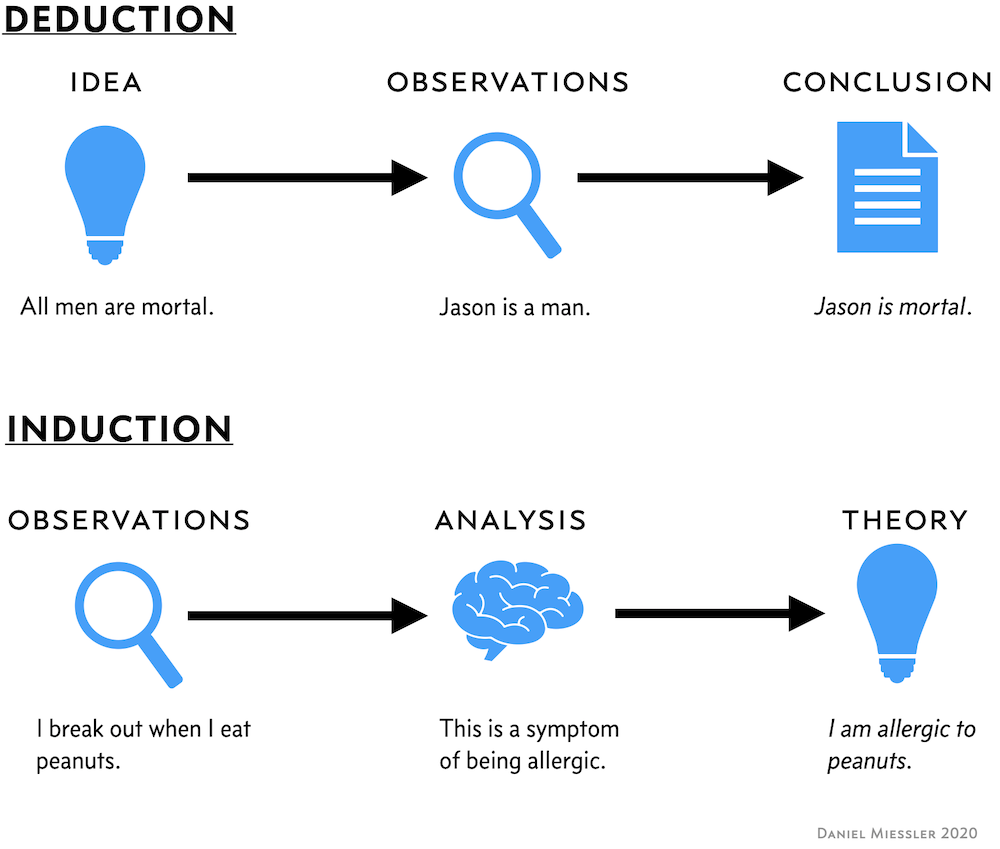
\includegraphics[width=0.7\textwidth]{Figure0101}
    \caption{Deduction vs. induction steps.}
    \label{lec_01_fig01}
\end{figure}

\begin{itemize}
    \item \textbf{Deduction}. Deductive reasoning is a process in which a conclusion follows logically from one or more premises. A \textit{premise} is a statement assumed to be true, often grounded in first principles or established theory. If the premises are true and the logical structure is valid, the conclusion is necessarily true.
    \[
    \text{Premise (Idea)} \;\rightarrow\; \text{Observation} \;\rightarrow\; \text{Conclusion}
    \]

    \item \textbf{Induction}. Inductive reasoning derives general principles from a collection of specific observations. These observations are assumed to be representative, and the resulting generalization is treated as empirical knowledge. Over time, validated inductive generalizations may evolve into accepted theories \footnote{It is important to distinguish \textit{mathematical induction} from \textit{inductive reasoning}. In a proof by mathematical induction (e.g., proving $1 + \dots + n = n(n+1)/2$), the argument is rigorous because it relies on the axioms of natural numbers.}.
    \[
    \text{Observation} \;\rightarrow\; \text{Analysis/Modeling} \;\rightarrow\; \text{Theory}
    \]

    \item \textbf{Abduction}. Abductive reasoning begins with an observation—often incomplete or surprising—and seeks the most plausible explanation. It is commonly described as "inference to the best explanation." Unlike deduction, abductive conclusions are not guaranteed.
    \[
    \text{Observation} \;\rightarrow\; \text{Hypothesis} \;\rightarrow\; \text{Evaluation}
    \]

    \item \textbf{Analogy}. Analogical reasoning draws inferences by identifying structural similarities between known and unknown situations, enabling hypothesis generation and conceptual transfer.
    \[
    \text{Known Case} \;\rightarrow\; \text{Comparison} \;\rightarrow\; \text{Inference about Unknown}
    \]
\end{itemize}

A crucial distinction between deductive and inductive reasoning lies in the certainty of their conclusions. Deductive reasoning yields conclusions that are true if the premises are true. Inductive reasoning, by contrast, produces conclusions that are \textit{probable}, as they rely on extrapolation from finite observations.



%In contrast, inductive reasoning in empirical contexts leads to generalizations that are inherently probabilistic. Such generalizations lack axiom-level guarantees and require \textit{verification} (checking consistency) and \textit{validation} (testing against real-world data). From a pessimistic view, inductive conclusions are never 100\% certain. Optimistically, however, inductive reasoning is indispensable: in the absence of complete information, it provides the best available basis for action.




These reasoning paradigms provide a useful conceptual framework for understanding modern AI algorithms. Although artificial systems do not reason in a human cognitive sense, many AI methodologies can be interpreted as computational analogues of these reasoning types. In practice, AI systems often combine multiple forms of reasoning within a single pipeline.

\begin{itemize}
    \item \textbf{Deductive reasoning} is reflected in rule-based systems and in the inference phase of trained models, where fixed premises (rules or learned parameters) are applied to new inputs to produce outputs.
    
    \item \textbf{Inductive reasoning} underlies most machine learning methods, including supervised, unsupervised, and reinforcement learning, where general patterns or policies are inferred from data or experience.
    
    \item \textbf{Abductive reasoning} appears implicitly in probabilistic modeling and generative systems, which infer plausible explanations or latent causes for observed data, particularly under uncertainty.
    
    \item \textbf{Analogical reasoning} emerges in representation learning and transfer learning, where knowledge acquired in one context is reused to solve structurally similar but previously unseen problems.
\end{itemize}

Last, it is noted that generative large models increasingly blur these boundaries, as rich internal representations enable behaviors that resemble abductive and analogical reasoning, even though the underlying computation remains fundamentally deductive at inference time.




\section{Classification of Modern AI and ML}
Despite this increasing convergence of reasoning behaviors in large-scale AI systems, it remains useful, particularly from an engineering and educational perspective, to introduce simplified classifications. % Such classifications do not imply sharp boundaries in real systems, nor do they imply that any single model belongs exclusively to a single category. 

% Instead, they serve as conceptual tools that isolate dominant design choices and computational mechanisms, enabling clearer understanding, comparison, and analysis. In the following sections, after discussing the relationship between ML and AI, we adopt several complementary classification schemes to organize modern AI and ML systems.

However, modern AI systems are complex artifacts that can be analyzed from multiple complementary perspectives. No single classification fully captures their behavior or design. In this section, we introduce several orthogonal lenses for organizing AI and ML systems, each emphasizing a different aspect: the relationship between learning and intelligence, the nature of system actions, the form of internal representations, and the scale at which learning occurs. Together, these perspectives provide a structured yet flexible framework for understanding contemporary AI.


\subsection{ML vs. AI}

We begin by classifying AI systems based on whether and how they acquire knowledge from data. Having established the types of reasoning associated with intelligence, we can now describe Artificial Intelligence (AI) and Machine Learning (ML) more precisely based on how they realize reasoning processes. 

First, we can view that AI, as a broad field, aims to create a process capable of emulating human intelligence or exhibiting intelligent behaviors. AI involves the design of agents that can perceive their environment, reason about it (using deductive, inductive, or other forms of logic), and take actions to achieve goals.

Second, we treat Machine Learning (ML) as a specific subset of AI focused on building models that learn from data (acknowledging that various definitions of ML exist \footnote{Definitions of ML vary across the field:
\begin{itemize}
    \item \textbf{Stanford University} defines ML as \href{http://mlclass.stanford.edu/}{"the science of getting computers to act without being explicitly programmed."} This broad definition suggests ML is the primary engine of modern AI.
    \item \textbf{Microsoft} defines ML as \href{https://azure.microsoft.com/en-us/resources/cloud-computing-dictionary/artificial-intelligence-vs-machine-learning}{"an application of AI; the process of using mathematical models of data to help a computer learn without direct instruction."}
\end{itemize}
}.

Most ML models implement the generic form of inductive reasoning: they learn from training data to acquire knowledge. When a trained model is used in practice, the process is called \textit{inference}. Inference, even though it is simply a calculation based on the trained model as a function, is effectively a generic form of a deductive process: the model is treated as a `true' premise, and it is applied to new inputs to derive a conclusion.


Specifically, Deep Learning is a further sub-branch of ML that utilizes multi-layered neural networks (see Fig.~\ref{lec_01_fig03}). Modern DL frameworks and models, by learning from and representing massive data (e.g., internet-scale data), achieve `generative' inference capabilities, including Large Language Models (LLMs), Large Vision Models (LVMs), and Large multi-modal Models (LMMs). 

\begin{figure}[htb]
         \centering
         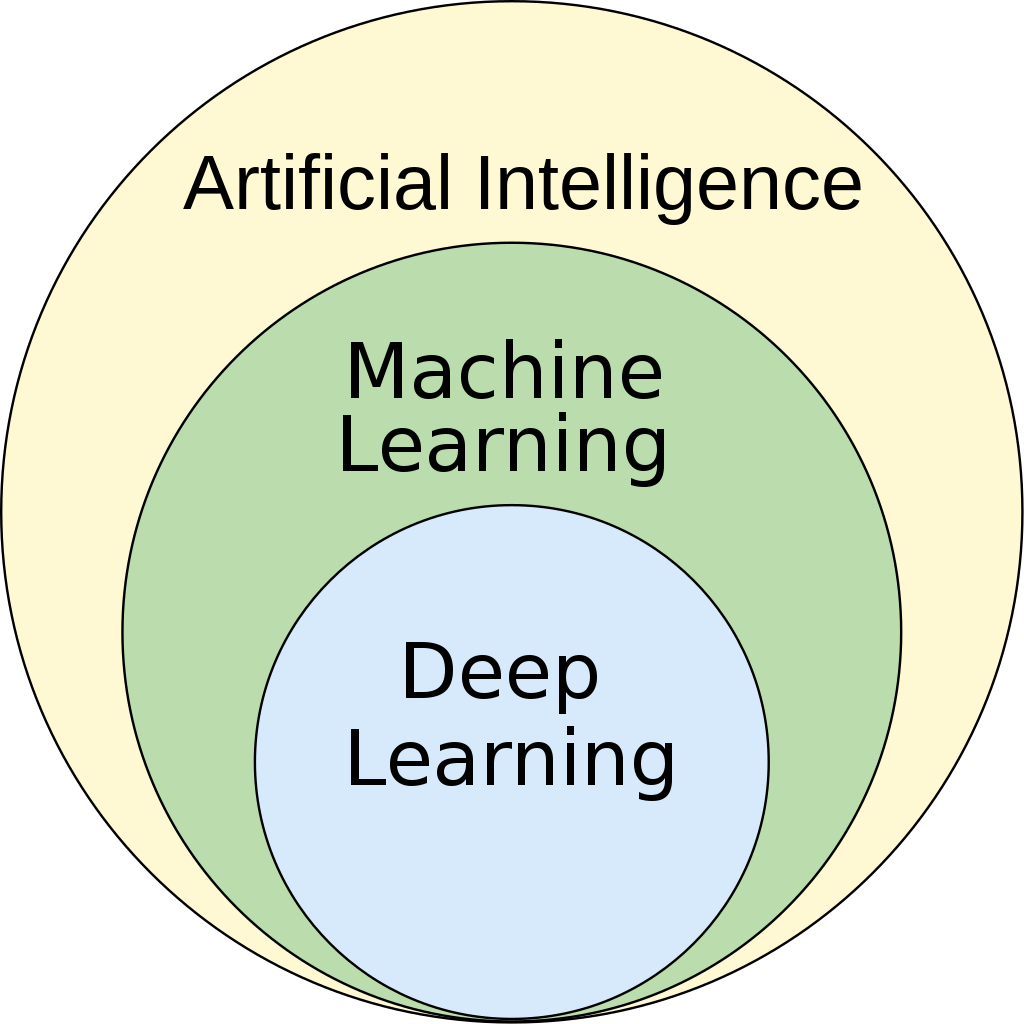
\includegraphics[width=0.4\textwidth]{Figure0103.png}
        \caption{AI and ML relations.}
        \label{lec_01_fig03}
\end{figure}


\subsection{Classification based on Action}
Next, we classify AI systems based on the nature of their actions and the role they play within a perception–inference–action pipeline. For engineers, it is helpful to view AI as a pipeline with four linked system components, other than merely action or feedback:
\emph{(i) Input}, \emph{(ii) representation}, \emph{(iii) inference}, and \emph{(iv) action}; subsequently, we classify AI based on the last phase - action - then understand the pipeline. 
\begin{itemize}
\item \textbf{Expert systems} emphasize explicit representations and logical inference. These systems typically lack a learning phase; intelligence is encoded by human design.
\item \textbf{Statistical machine learning (ML) systems} emphasize learning inference rules from data, requiring training and validation.
\item \textbf{Deep learning systems}, as a branch of ML systems, strengthen representation learning, enabling hierarchical feature discovery from raw data, including large language models (LLMs) as a major breakthrough.
\item \textbf{Agentic AI systems} emphasize system-level integration rather than a new AI paradigm. They combine pretrained foundation models with mechanisms for planning, tool use, memory, and interaction with the environment. While classical AI agents and reinforcement learning systems have long studied sequential decision-making, recent agentic systems leverage large pretrained models as flexible world priors, enabling rapid task specification and coordination across tools. The resulting behavior may appear autonomous, but agency remains externally defined by system design and objectives.
\end{itemize}

\paragraph{Toward Embodied Intelligence.} Despite recent advances in agentic AI systems, the role of action in contemporary AI remains fundamentally limited. In most current systems, actions, whether tool calls, control signals, or generated plans, are treated as one-way executions whose consequences are not intrinsically coupled back into the learning or objective structure of the model. Feedback from action is typically externalized, episodic, or manually curated, rather than forming a persistent, self-driven interaction loop. 

As a result, these systems lack core properties of embodied intelligence, such as survival-driven behavior, autonomous exploration, and continual adaptation through closed-loop perception–action coupling. Bridging this gap by tightly integrating action, feedback, and internal world models represents a transformative shift in AI paradigms, moving beyond task execution toward genuinely embodied and self-sustaining intelligence.



\subsection{Classification based on Representation}
Another fundamental distinction arises from how knowledge and uncertainty are represented internally within the system.

\begin{itemize}
    \item \textbf{Symbolic Formulation} represents knowledge explicitly using logical rules and symbols. Intelligence is encoded manually by human experts. The system itself does not learn from data; instead, humans perform the inductive reasoning externally to create the rules. During execution, the system performs pure deductive reasoning. These systems are transparent but often brittle in the face of uncertainty.

    \item \textbf{Supervised Learning} is a data-driven inductive process in which a model learns from labeled examples (input-output pairs). The objective is to learn a function that maps inputs to outputs by minimizing error. Once trained, the model is fixed, and inference proceeds deductively.

    \item \textbf{Unsupervised Learning}  aims to discover latent structure in unlabeled data, such as clusters or probability distributions. It is a form of unsupervised induction, often used to create representations for downstream tasks.



    \item \textbf{Reinforcement Learning (RL)} introduces a fundamentally different learning setting in which an agent acquires behavior through continual interaction with an environment. Unlike supervised or unsupervised learning, which rely on static datasets, RL couples perception, decision-making, and action within a feedback loop driven by reward signals. Through exploration and trial-and-error, the agent inductively learns a policy, which is then applied deductively to select actions over time.
    
    Conceptually, RL represents the closest classical AI framework to embodied intelligence, as it explicitly models action, consequence, and delayed feedback. However, most practical RL systems remain limited to narrowly defined environments, externally specified rewards, and short or moderate time horizons. They lack intrinsic survival objectives, persistent world models, and open-ended adaptation, which are hallmarks of biological intelligence.

\end{itemize}

\subsection{Classification based on Scale}
Finally, we consider classification based on scale, which has emerged as a dominant factor shaping modern AI capabilities and system behavior.

Although the classic representation and learning formalisms have largely remained unchanged to date, and the goal of AI actions has remained the same, the scale of AI has dramatically transformed. Today, AI models are simply separated into small and large models - the latter is termed `Foundation AI Models'. The emergence of foundation models, such as Large Language Models (LLMs), has altered our perspective on learning and inference. Unlike classical models trained for narrow tasks and small datasets, or developed based on a limited set of symbolic rules, foundation models are trained on massive and diverse datasets, learning general representations applicable to thousands of downstream tasks.

At the inference time, foundation models appear to perform inductive reasoning: they adapt to new tasks and generate novel outputs from minimal prompting (in-context learning). However, strictly speaking, the model parameters remain fixed. The model is performing a complex form of deductive inference over a highly rich internal representation.

What has changed is the \textit{scope} of induction. Foundation models perform induction at an unprecedented scale during training, compressing vast amounts of "world knowledge" into their parameters. This allows their inference behavior to resemble \textit{abduction} (guessing intent) and \textit{analogy} (transferring patterns), even though the underlying computation is deterministic.

\paragraph{Final Note.} It is important to note that a single AI system may simultaneously belong to multiple categories under different lenses. For example, a large language model can be viewed as a deep learning system, a foundation model, a statistical inductive learner, and a component within a larger agentic system. These classifications are not mutually exclusive but highlight different design and analysis priorities.


\section{Conclusions and Forward Looking}
This chapter established a conceptual landscape for Artificial Intelligence by situating modern AI systems within the broader spectrum of natural and cognitive intelligence. By examining organisms ranging from single-celled life to higher primates, we emphasized that intelligence is multifaceted, embodied, and tightly coupled to interaction with the physical world. In contrast, contemporary AI systems primarily realize intelligence through formalized reasoning and statistical learning, achieving remarkable performance in constrained domains while lacking intrinsic agency and closed-loop embodiment.

Within this landscape, we highlighted deduction and induction as the dominant reasoning processes underlying modern AI. Most data-driven systems rely on large-scale inductive learning during training and deductive computation during inference. Although recent foundation models blur traditional boundaries and exhibit behaviors resembling abduction and analogy, their core computational mechanisms remain grounded in statistical (inductive) learning and (deductive) inference.

Accordingly, this course adopts a primarily statistical perspective on AI. We will focus on the formalisms of supervised and unsupervised learning that constitute data-driven machine learning, including the study of learning mechanisms, generalization, and quantitative evaluation of inference-phase performance. These methods dominate modern AI systems in both industrial and scientific applications and form the technical foundation upon which large-scale models are built.

Symbolic AI and reinforcement learning are treated as essential but secondary components. Symbolic methods provide conceptual clarity and interpretability, while reinforcement learning introduces action, feedback, and interaction. Although they are not the primary focus, both paradigms are revisited where they inform system design and decision-making.

Finally, consistent with an engineering emphasis on action, this course treats modern generative models as enabling infrastructure rather than objects of study in isolation. We take large pretrained models as given and focus instead on how they are used: how learned representations support decision-making, how inference quality is evaluated, and how generative AI can be integrated into agentic processes. Through hands-on practice, students will learn to design, implement, and reason about AI systems that act—bridging learned models with tools, environments, and objectives.


\end{document}